\phantomsection\numberedsection{RF2.2 Editar Producto}

\subsection*{Descripción}
Los usuarios deben de poder modificar los atributos relacionados con cualquier producto.\par
\vspace{0.15cm}

\textbf{Pre-condición}\par
El usuario debe haber iniciado sesión en su cuenta en Mini PIM y haber creado al menos un producto.\par
\vspace{0.15cm}

\textbf{Post-condición}
\begin{itemize}
    \item Caso de éxito: En el producto se reflejan los cambios realizados por el usuario.
    \item Caso mínimo: El sistema notifica al usuario el resultado de la accion editar producto; exitosa o fallida.
\end{itemize}

\textbf{Prioridad: }
Alta
\vspace{0.15cm}

\textbf{Autor: }
Angel Nicolas Escaño Lopez\par
\vspace{0.15cm}

\textbf{Control de cambios: } Versión 1: Definición del caso de uso

\numberedsubsection{Escenario principal}
\begin{enumerate}
    \item El usuario se encuentra en productos y tras seleccionar uno de ellos en el \textit{DataGrid}, hace clic en el icono de \enquote{Editar Producto}.
    \item El sistema muestra los atributos del producto editable.
    \item El usuario selecciona los atributos que desea editar y los rellena.
    \item El sistema comprueba la validez de los datos introducidos por el usuario.
    \item El sistema almacena los atributos del producto seleccionados por los nuevos que ha dado el usuario en la base de datos.
    \item El sistema modifica la información de dichos atributos en la base de datos del sistema.
    \item El sistema muestra los cambios y notifica al usuario de la finalización de la operación con éxito.
\end{enumerate}

\numberedsubsection{Escenarios alternativos}
\begin{description}
    \item[2.a.] El usuario cancela la opción de edición de atributos de productos seleccionando la opción de cerrar menu de edición.
    \begin{enumerate}
        \item[2.a.1] El sistema regresa al usuario al apartado de visualización de productos.
    \end{enumerate}

    \item[3.a] El sistema detecta un fallo en la comprobación de los atributos a modificar.
    \begin{enumerate}
        \item[3.a.1] El fallo se detecta porque el campo esta en nulo.
        \item[3.a.2] El fallo se detecta porque ha sobrepasado los limites de caracteres.
        \item[3.a.3] El fallo se detecta porque el campo contiene caracteres ilegales.
        \item[3.a.4] El fallo se detecta porque el tipo de dato introducido es incorrecto.
        \item[3.a.5] El sistema notifica del error al usuario mostrando en que dato se produjo el error.
        \item[3.a.6] El sistema regresa al menu de productos permitiendo la edición de los datos.
    \end{enumerate}
\end{description}

\numberedsubsection{Casos de Prueba}
\underline{Escenario: Principal}\par
\vspace{0.15cm}
\textbf{Dado} que hay al menos un producto creado,\par
\textbf{Y} estoy en el apartado de Productos,\par
\textbf{Cuando} selecciono la opción de \enquote{Editar},\par
\textbf{E} introduzco correctamente los atributos que deseo editar,\par
\textbf{Y} Selecciono \enquote{Confirmar} para guardar los cambios,\par
\textbf{Entonces} el sistema almacena la información en la base de datos de Mini PIM,\par
\textbf{Y} modifica la información del producto a editar en la base de datos,\par
\textbf{Y} muestra el apartado de visualización de productos con el producto editado.\par
\vspace{0.20cm}

\underline{Escenario: Alternativo 2.a}\par
\vspace{0.15cm}
\textbf{Dado} que hay un producto creado,\par
\textbf{Y} estoy en el apartado de visualización de productos,\par
\textbf{Cuando} selecciono la opción de \enquote{Editar},\par
\textbf{Y} selecciono la opción de \enquote{Cancelar},\par
\textbf{Entonces} el sistema muestra el apartado de visualización de productos mostrando todos los recursos almacenados sin ningún cambio.\par
\vspace{0.20cm}

\underline{Escenario: Alternativo 3.a}\par
\vspace{0.15cm}
\textbf{Dado} que hay un producto creado,\par
\textbf{Y} estoy en el apartado de visualización de productos,\par
\textbf{Cuando} selecciono la opción de \enquote{Editar},\par
\textbf{Y} escribo los datos del atributo y dejo uno obligatorio vacío, supera el límite de caracteres o contiene caracteres ilegales o inserto un tipo de dato incorrecto,\par
\textbf{Entonces} el sistema me muestra cual es el atributo que falla,\par
\textbf{Y} regresa al apartado de visualización de atributos de productos sin modificaciones.\par
\vspace{0.20cm}

\numberedsubsection{Bocetos}

\begin{figure}[H]
    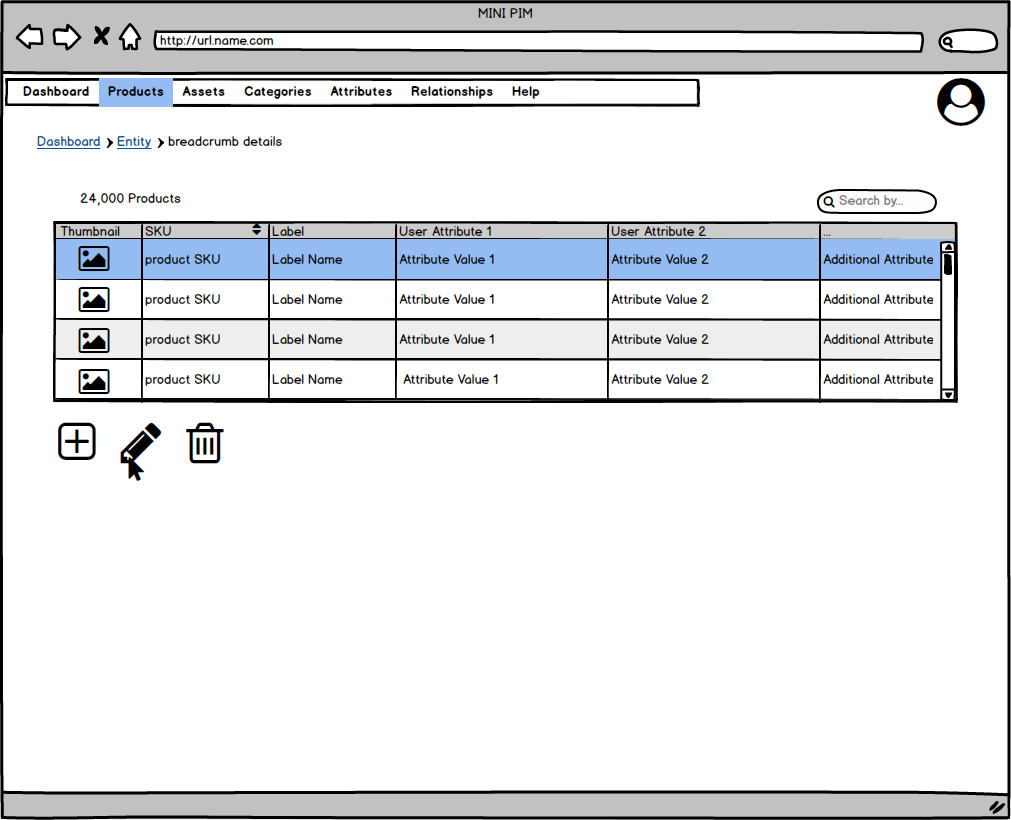
\includegraphics[width=1\linewidth]{mockups/RF2-X Editar Producto Click en Lapiz.png}
    \caption{Edición de Productos hacer clic en \enquote{Editar}}
   \end{figure}
\vspace{1.0cm}


\begin{figure}[H]
    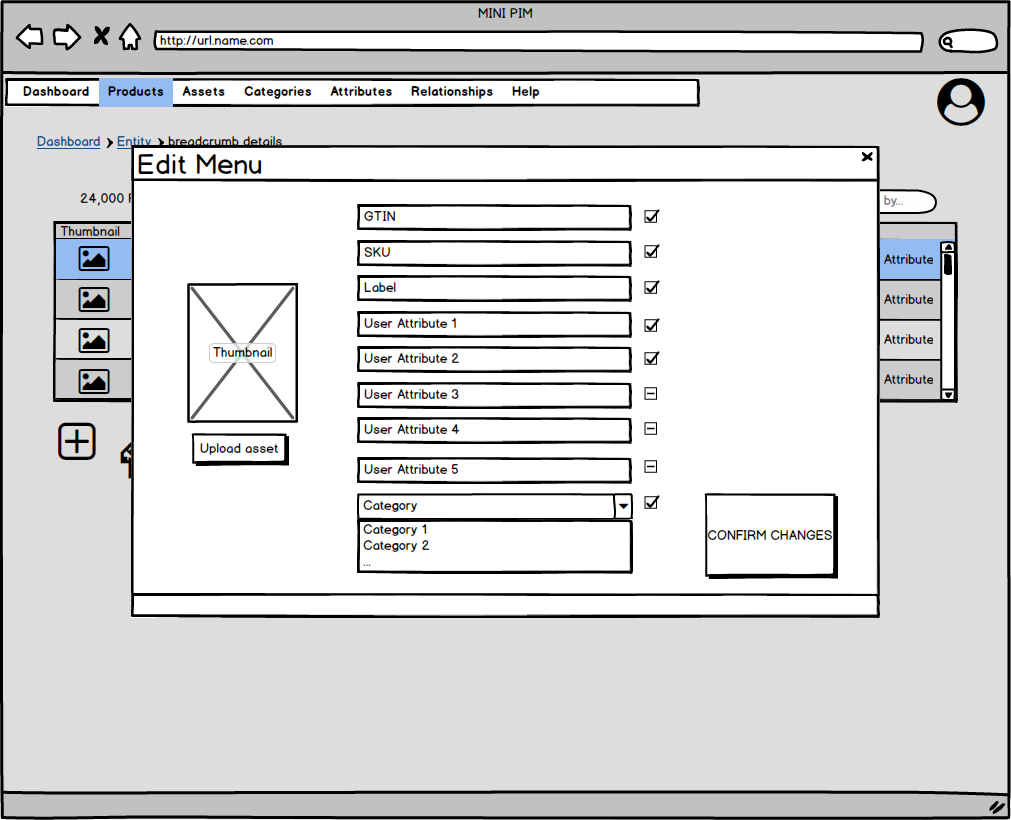
\includegraphics[width=1\linewidth]{mockups/RF2-X Editar ProductoV2.png}
    \caption{Edición de Productos tras clicar \enquote{Editar}}
   \end{figure}
\vspace{1.0cm}

\newpage %Inicia en una nueva página otro caso de uso